% =====================
% Chapter 5: Booleans (Detailed)
% Audience: Architecture students new to coding
% =====================

\h{Booleans}
In the programming, we constantly need to ask questions and make decisions based on the answers. Is a building's height over the city's limit? Does a room's area meet the client's minimum requirement? Is the selected material steel? The answers to these questions are not numbers or strings of text; they are simple "yes" or "no" assertions. In Python, this concept of "yes" or "no" is represented by a data type called a Boolean. There are only two possible Boolean values: True and False. Notice that they are capitalized. These are special keywords in Python that represent the state of a condition. True is the equivalent of "yes, this is correct," and False is the equivalent of "no, this is incorrect."
\medskip
\begin{NoteBox}
\textbf{About this chapter.}
Booleans represent truth values: \c{True} or \c{False}. They power conditions in \c{if},
filtering, validation, and control flow. We cover Boolean literals, truthiness, comparisons,
logical operators (with short-circuit), precedence, membership tests, guard patterns,
and common pitfalls you’ll meet in practice.
\end{NoteBox}
\medskip

\begin{tcolorbox}[% passing options here
    title=Focus of this chapter:,
    colframe=orange,
    colback = white,
%    colback=orange!40!yellow!30, % think of mixing 2 colors with sliders
    arc=2mm % sharp corners
 ]
\begin{itemize}
  \item Boolean basics: \c{True}, \c{False}, and the \c{bool} type; Booleans as a subtype of \c{int}.
  \item Truthiness: which values act as false (\c{0}, \c{""}, \c{[]}, \c{{}}, \c{None}) vs true.
  \item Comparisons: \c{==}, \c{!=}, \c{<}, \c{<=}, \c{>}, \c{>=}; chained comparisons like \c{3 < x <= 10}.
  \item Logical operators: \c{not}, \c{and}, \c{or} with short-circuit evaluation and precedence.
  \item Membership tests: \c{in}, \c{not in} for strings and lists.
  \item any/all: quick checks across collections.
  \item Identity and None: use \c{is} / \c{is not} with \c{None}; prefer \c{==} for value equality.
  \item Guard patterns: validate and convert input safely; boolean expressions for clean filters.
  \item Pitfalls: \c{=} vs \c{==}, \c{is} vs \c{==}, floats in comparisons (\c{math.isclose}), using \c{&}/\c{|} by mistake, and the \emph{``or-membership''} bug.
\end{itemize}
\end{tcolorbox}

\hh{Why Booleans matter}
Booleans are control signals for your code: they gate rules, filters, and validation.
They make small design scripts readable and correct (e.g., “is area within limits?”).

\hh{Boolean literals and type}
\c{True}/\c{False} values, the \c{bool} type, and how booleans behave like 1/0 in arithmetic.

\code{c06_literals}{python}{
    a = True
    b = False
    print(type(a))     # <class 'bool'>
    print(a + 1)       # 2 (True behaves like 1; False like 0)
}{Booleans are True or False; they behave like 1 and 0 in arithmetic.}

\hh{Truthiness: which values count as False}
Empty strings/lists/dicts and zero-like numbers evaluate to False; others are True.
Use \c{bool(x)} to preview how \c{x} behaves in a condition.

\code{c06_truthiness}{python}{
    print(bool(0), bool(0.0), bool(0j))   # False False False
    print(bool(""), bool([]), bool({}))   # False False False
    print(bool(None))                     # False
    print(bool(5), bool("Lobby"))         # True True
}{Empty or zero-like values are False; non-empty or non-zero values are True.}

\hh{Comparisons produce booleans}
Relational/equality operators return \c{True} or \c{False}; chained comparisons read like math.

\code{c06_comparisons}{python}{
    print(10 > 9)                 # True
    print(10 == 9)                # False
    print("Lobby" == "Lobby")     # True
    print(3 < 5 <= 5)             # True (chained comparison)
}{Relational and equality operators return True or False.}

\hhh{Chained comparisons}
Write \c{min < x <= max} instead of \c{min < x and x <= max}.

\code{c06_chained}{python}{
    span_m = 7.2
    ok = 6.0 <= span_m <= 9.0     # between 6 and 9 inclusive
    print(ok)                     # True
}{Chaining reads like math and is less error-prone.}

\hh{Logical operators: not, and, or}

\begin{figure}[htbp]
  \centering
  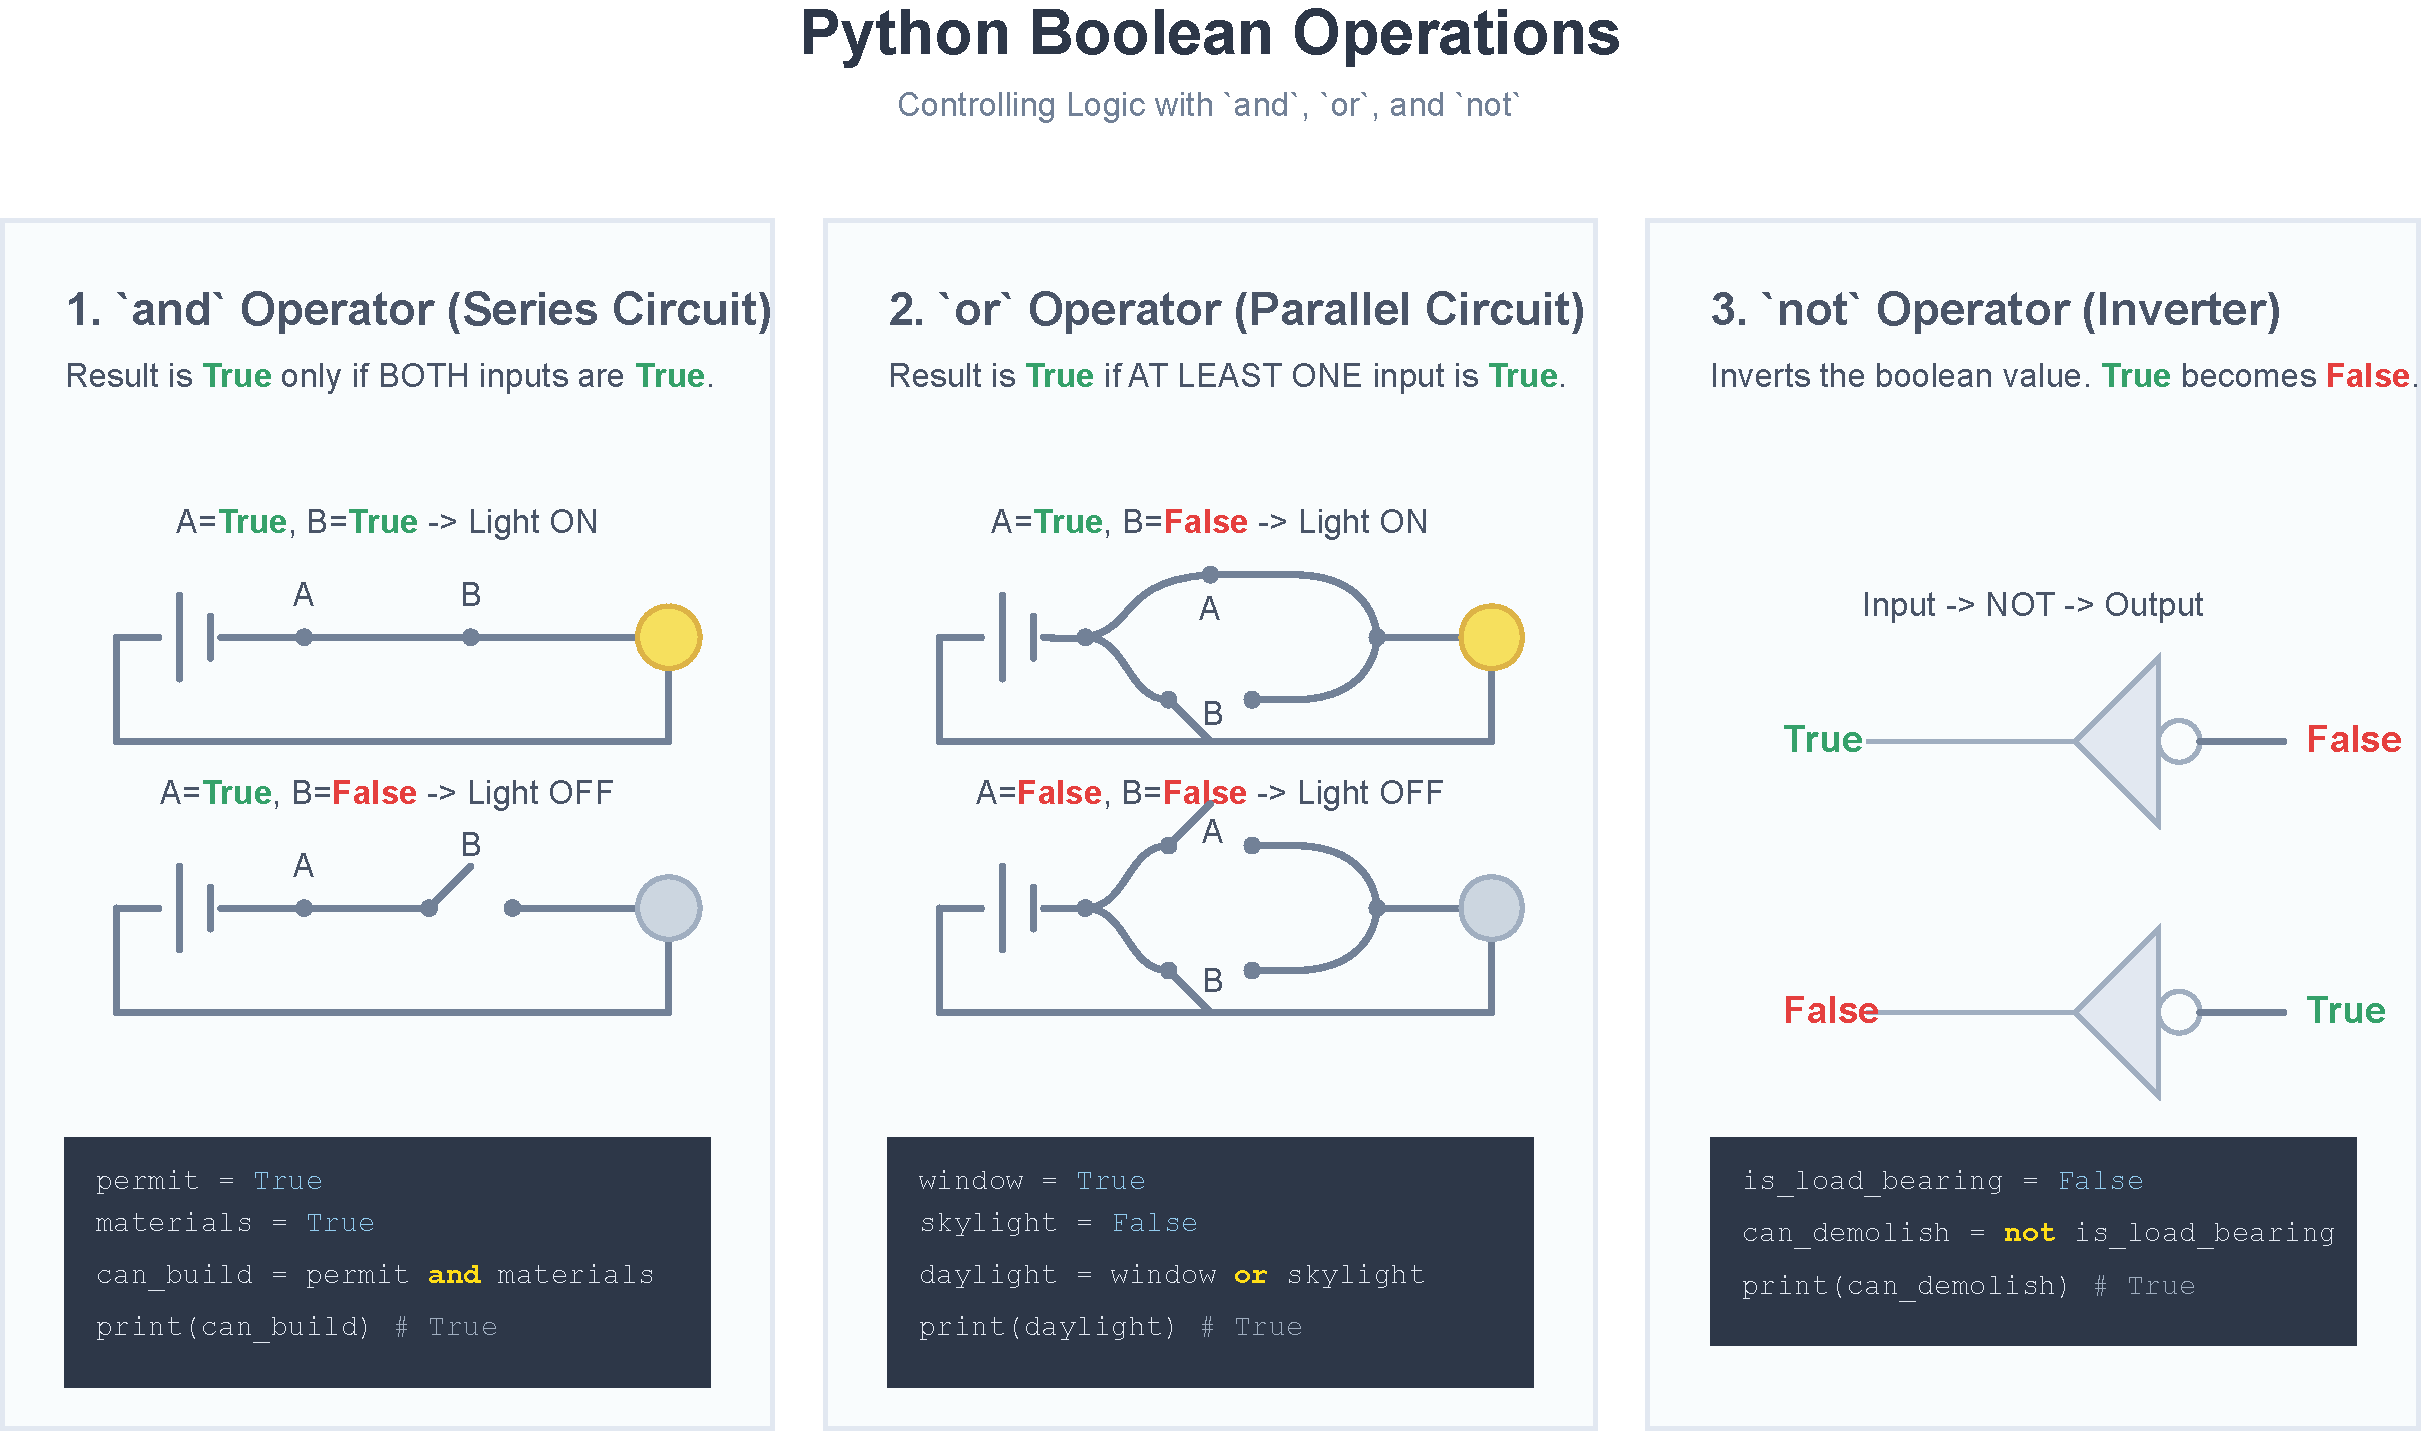
\includegraphics[width=0.85\linewidth]{Figures/Boolean/Boolean_operation.pdf}
  \caption{Boolean operations.}
  \label{fig:boolean-operations}
\end{figure}

Combine conditions using \c{not}, \c{and}, and \c{or}. Remember: \c{not} binds tightest, then \c{and}, then \c{or}.

\code{c06_logic}{python}{
    w = 3.0
    l = 5.0
    area_ok = (w * l) >= 15.0
    named   = "Lobby" != ""

    print(not area_ok)            # invert
    print(area_ok and named)      # both must be True
    print(area_ok or named)       # at least one is True
}{Logical operators combine boolean expressions.}

\hhh{Operator precedence (important)}
Order is: \c{not} \(\rightarrow\) \c{and} \(\rightarrow\) \c{or}. Use parentheses to be explicit.

\code{c06_precedence}{python}{
    a, b, c = True, False, True
    print(a or b and c)       # and runs before or -> True
    print((a or b) and c)     # parentheses can change meaning
    print(not a or b)         # not runs before or
}{not > and > or. Add parentheses when in doubt.}

\hhh{Short-circuit behavior}
\c{and} stops early when the left side is False; \c{or} stops early when the left side is True.
They return one of their operands (not necessarily a literal True/False).

\code{c06_short_circuit}{python}{
    user = ""
    # pick a default label when user is empty
    label = user or "Unnamed"     # returns right side if left is falsy
    print(label)                  # "Unnamed"

    # safe numeric: don't use "or" with numbers (0.0 is falsy!)
    w = 0.0
    l = 4.0
    ratio = (l / w) if w else None   # None means "not defined"
    print(ratio)                     # None (no ZeroDivisionError)
}{Use short-circuiting for defaults and to avoid unnecessary work.}

\hh{Membership tests: in / not in}
Test containment in strings or collections.

\code{c06_in}{python}{
    materials = ["concrete", "steel", "wood"]
    print("steel" in materials)        # True
    print("glass" not in materials)    # True

    name = "Lobby"
    print("bb" in name)                # True (substring)
}{Use membership tests for clean, readable checks.}

\hh{any and all for collections}
Aggregate boolean checks: \c{any} for “at least one”, \c{all} for “every item”.

\code{c06_any_all}{python}{
    spans = [6.0, 7.2, 8.4]
    print(any(s >= 8.0 for s in spans))             # True if at least one meets the condition
    print(all(6.0 <= s <= 9.0 for s in spans))      # True if every span in [6, 9]

    # Counting True values works because bools are 1/0
    checks = [s >= 6.5 for s in spans]
    print(sum(checks))                               # count how many pass
}{Use any/all to evaluate many items succinctly.}

\hh{Identity and None}
Compare with \c{None} using \c{is}; use \c{==} for values. For floats, use a tolerance.

\code{c06_none_isclose}{python}{
    import math

    height = None
    if height is None:
        print("Height not set")

    name = "Lobby"
    print(name == "Lobby")                 # value comparison (correct)
    # print(name is "Lobby")               # avoid 'is' for strings

    span = 7.2
    est  = 0.1 + 7.1
    print(est == span)                     # may be False due to float rounding
    print(math.isclose(est, span, rel_tol=1e-9, abs_tol=1e-12))  # robust
}{Use 'is' with None; prefer math.isclose for float equality.}

\hh{Guard patterns and validation}
Use guards to validate inputs before conversion or computation.

\code{c06_guard}{python}{
    txt = input("Width (m): ").strip()
    if not txt:                      # empty string -> invalid
        print("Please enter a number")
    else:
        try:
            w = float(txt)
            print("OK:", w)
        except ValueError:
            print("Not a valid number")
}{Use boolean guards to validate before converting.}

\hh{Common pitfalls and how to avoid them}
\c{=} vs \c{==}, \c{is} vs \c{==}, float comparisons, bitwise vs logical, and the or-membership bug.

\begin{itemize}
  \item Assignment vs equality: \c{=} assigns, \c{==} compares. \c{if x = 3} is a syntax error; write \c{if x == 3}.
  \item \c{is} vs \c{==}: use \c{is} for identity (\c{None}), not for strings or numbers.
  \item Floats: prefer a tolerance check or \c{math.isclose(a, b)} instead of \c{a == b}.
  \item Bitwise \c{&} and \c{|} vs logical \c{and}/\c{or}: write \c{and}/\c{or} for booleans.
  \item Or-membership bug: \c{if tag == "NORTH" or "SOUTH":} is \emph{always} True.
\end{itemize}

\code{c06_or_bug}{python}{
    tag = "NORTH"
    print(tag == "NORTH" or "SOUTH")          # BUG: always True
    print(tag in ("NORTH", "SOUTH"))          # Correct
}{Use 'in' for one-of checks.}

\hhh{De Morgan's laws (refactor negatives)}
\c{not (A and B)} \(\equiv\) \c{(not A) or (not B)} and \c{not (A or B)} \(\equiv\) \c{(not A) and (not B)}.

\code{c06_demorgan}{python}{
    w, l = 0.0, -1.0
    bad  = not (w > 0 and l > 0)
    good = (w <= 0) or (l <= 0)
    print(bad == good)   # True
}{Turn a big negative into clearer positive pieces.}

\hh{Worked example: room filters with rules}

\begin{NoteBox}
\textbf{What this shows.} Express multiple constraints by naming booleans and combining them with \c{and}.
\end{NoteBox}

\code{c06_worked}{python}{
    rooms = [
        {"room": "101", "area_m2": 18.5, "occupied": True},
        {"room": "102", "area_m2": 21.0, "occupied": False},
        {"room": "103", "area_m2": 17.2, "occupied": True},
    ]

    # keep rooms that are occupied AND area at least 18.0
    selected = [
        r for r in rooms
        if r["occupied"] and r["area_m2"] >= 18.0
    ]

    # report if any room is below 18.0
    any_small = any(r["area_m2"] < 18.0 for r in rooms)
    print(selected, any_small)
}{Combine comparisons, and/or, any/all in practical filters.}

\hh{Mini-Lab A: validation and reporting}
Prompt for \c{width} and \c{length}. If either input is empty or not numeric, print an error.
Otherwise compute \c{area} and print whether \c{18.0 <= area <= 30.0}. Then print \c{OK} if
both width and length are positive numbers; else print \c{Not OK}.

\code{c06_mini_lab_scaffold}{python}{
    # 1) Read and validate
    w_txt = input("Width (m): ").strip()
    l_txt = input("Length (m): ").strip()

    if not w_txt or not l_txt:
        print("Please enter both width and length.")
    else:
        try:
            w = float(w_txt)
            l = float(l_txt)
        except ValueError:
            print("Inputs must be numbers.")
        else:
            # 2) Compute and report
            area = w * l
            in_range = 18.0 <= area <= 30.0
            ok_dims  = (w > 0) and (l > 0)

            print(f"Area = {area:.2f} m\u00B2")
            print("Area in [18, 30]? ", in_range)
            print("Dimensions positive? ", ok_dims)
            print("Overall:", "OK" if (in_range and ok_dims) else "Not OK")
}{Scaffold to practice boolean validation and reporting}

\hh{Self-check}
\begin{itemize}
  \item Explain short-circuit evaluation in your own words and give one safe-default example using \c{or}.
  \item Rewrite \c{6 < x and x < 12} using a chained comparison.
  \item Show a tolerance-based float comparison that checks if \c{span} is effectively 7.2.
  \item When should you use \c{is} vs \c{==}? Give two examples.
\end{itemize}
